\section{2点関数\label{sec:twopointfunc}}
ここではラージ$N$におけるSYK模型の2点関数について述べる。
最初に2点関数の従うシュウィンガー・ダイソン方程式を示し, そこから
リーディングオーダーで寄与するファインマンダイアグラムがメロンダイアグラムと呼ばれる
ものである事を見る。

次にシュウィンガー・ダイソン方程式が低エネルギー極限でリパラメトリゼーション不変性を
持つ事を見る。
この不変性は, 古典解として共形対称性を持つものを選ぶ事によって自発的に破れる。
この共形古典解を用いて, 第\ref{sec:fourpointfunc}節で4点関数の解析を行う。

シュウィンガー・ダイソン方程式の解析解は共形古典解の他にも, 
相互作用するフェルミオンの数$q$についてラージ極限を取ったものや, $q=2$の時にも知られている. 
ただし本論文では$q=2$のケースは重要ではないので扱わない. 

なおこの節以降では, ある関数$f$のフーリエ変換を$F[f]$と表記する:
\begin{align}
	F[f](\omega) \equiv \int dt\ e^{i\omega t}f(t).
\end{align}

\subsection{シュウィンガー・ダイソン方程式}
\begin{figure}[ht]
  \centering
  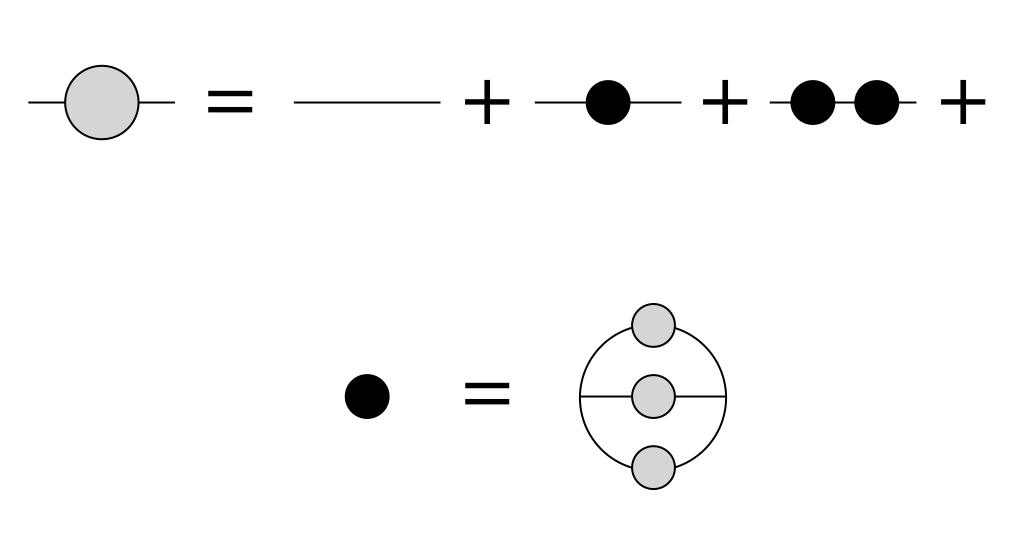
\includegraphics[width=14cm]{figures/melonDiagram}
  \caption{ラージ$N$極限において2点関数に寄与する最初の補正ダイアグラム.
  特に$q=4$の場合について描画している. 灰色の丸と黒い丸はそれぞれ完全な2点関数および
  1粒子相互作用を表している.}
  \label{fig:melonDiagram}
\end{figure}

SYK模型の作用は
\begin{align}
  I = \int dt\ \left(\frac{1}{2}\sum_{i = 1}^{N} \psi_i \deriv \psi_i
		- \frac{1}{4!} \sum_{i,j,k,l = 1}^{N} J_{ijkl} \psi_i\psi_j\psi_k\psi_l
    \right)
\end{align}
である. 
これを$J_{ijkl}$について期待値を取り, その後フェルミオンを積分するために
2つの双局所場$G(t_1, t_2)$, $\Sigma(t_1, t_2)$を導入すると
\begin{align}
  \frac{I_{\mathrm{eff}}}{N} =
		- \frac{1}{2}\log\det\left(\deriv - \Sigma\right)
		+ \frac{1}{2}\int dt_1dt_2\ \left(\Sigma G - \frac{J^2}{4}G^4\right)
  \label{eq:effectiveAction}
\end{align}
を得る\footnote{詳しい計算は\ref{app:effective_action}を参照すること.}. 
$\Sigma$は$G = \frac{1}{N}\sum_j \psi_j(t_1)\psi_j(t_2)$とするような
ラグランジュの未定乗数である. 
\eqref{eq:effectiveAction}式の停留点が次式のシュウィンガー・ダイソン方程式を与える:
\begin{align}
  F[G](\omega)^{-1} = -i\omega - F[\Sigma](\omega),
  \hspace{30pt}
  \Sigma(t) = J^2G(t)^3.
  \label{eq:SDeq}
\end{align}

なお, SYK模型では4つのフェルミオンが相互作用するとしているが, その数を$q$として一般化しても
作用を書く事ができ,
\begin{align}
	I = \int dt\ \left(
		\frac{1}{2}\sum_{i = 1}^N \psi_i\deriv \psi_i	
		- i^{q/2}\sum_{1\leq i_1 < i_2 < \cdots < i_q \leq N}J_{i_1i_2\cdots i_q}\psi_{i_1}\psi_{i_2}\cdots\psi_{i_q}
	\right)
\end{align}
である.
同様に有効作用やシュウィンガー・ダイソン方程式も計算する事ができ, それぞれ
\begin{align}
  \frac{I_{\mathrm{eff}}}{N} =
		- \frac{1}{2}\log\det\left(\deriv - \Sigma\right)
		+ \frac{1}{2}\int dt_1dt_2\ \left(\Sigma G - \frac{J^2}{q}G^q\right),
  \label{eq:effectiveActionWithGeneral_q}
\end{align}
\begin{align}
  F[G](\omega)^{-1} = -i\omega - F[\Sigma](\omega),
  \hspace{30pt}
  \Sigma(t) = J^2G(t)^{q-1}
  \label{eq:SDeqWithGeneral_q}
\end{align}
である. さらに複数の$q$について相互作用項を足し合わせたような一般化したSYK模型も
調べられており, \cite{gross}にて詳しく論じられている. 

ラージ$N$極限を施したSYK模型において, リーディングオーダーで2点関数に寄与する
ファインマンダイアグラムは「メロンダイアグラム」と呼ばれている. 
\eqref{eq:SDeqWithGeneral_q}式の一般の$\omega$における解析的な計算は現在のところ
知られていないが, 数値的には可能であり, 図\ref{fig:melonDiagram}のダイアグラムのように
再帰的に計算を走らせる事で2点関数のグラフをプロットできる(図\ref{fig:J10}, 図\ref{fig:J50}). 

\begin{figure}[ht]
	\begin{tabular}{cc}
		\begin{minipage}[t]{0.45\hsize}
			\centering
			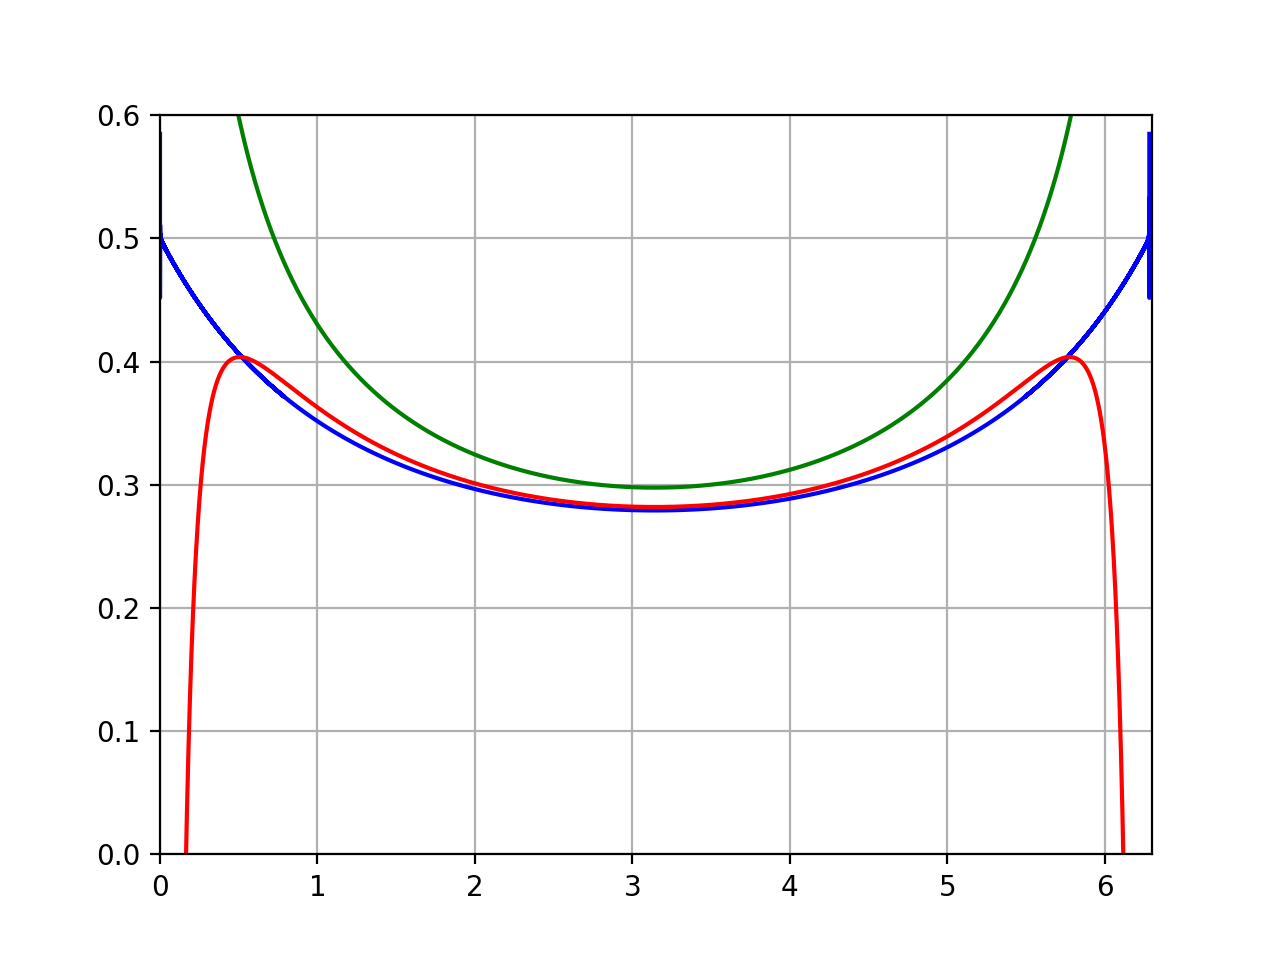
\includegraphics[width=8cm]{figures/J10}
			\caption{$J = 10$としてプロットした2点関数. 横軸は時間である. 
			青色の線が一般の$\omega$, 緑色の線が$\omega = 0$, 
			赤色の線が低エネルギー極限に$J^{-1}$補正を加えたものである.}
			\label{fig:J10}
		\end{minipage}
		\begin{minipage}[t]{0.45\hsize}
			\centering
			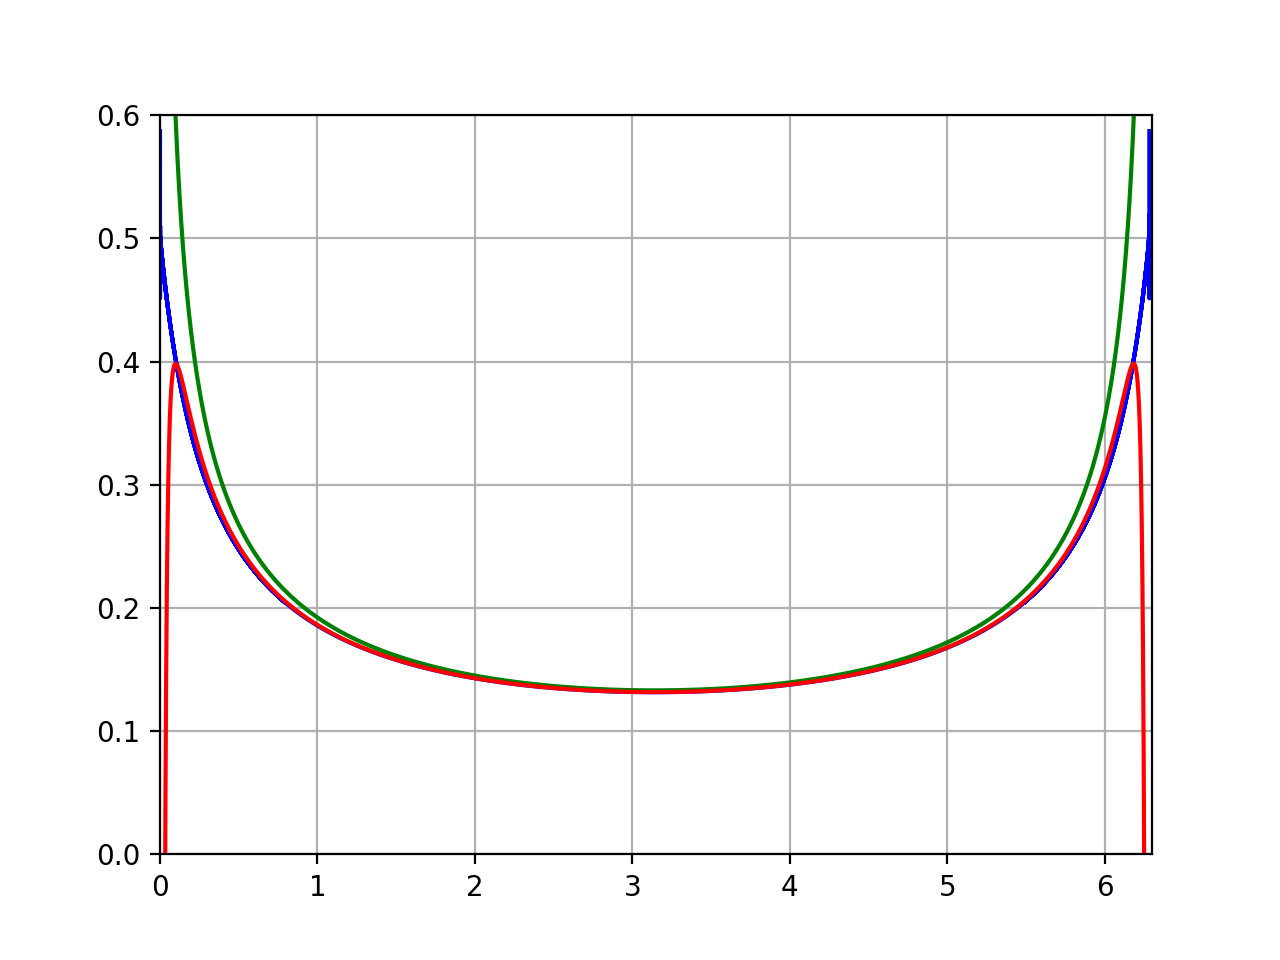
\includegraphics[width=8cm]{figures/J50}
			\caption{$J = 50$としてプロットした2点関数. 横軸は時間である. 各色の意味は左図と同様. 
				低エネルギー極限はラージ$J$極限でもあるので, 左図と比べて各線は互いに近づく.}
			\label{fig:J50}
		\end{minipage}
	\end{tabular}
\end{figure}

\subsection{共形不変性}
シュウィンガー・ダイソン方程式\eqref{eq:SDeqWithGeneral_q}は$\omega = 0$という
低エネルギー極限においては解析的な解が知られている. 
この時\eqref{eq:SDeqWithGeneral_q}式の一つ目の式は
\begin{align}
	F[\Sigma](\omega)F[G](\omega) = -1
\end{align}
となり, この両辺にフーリエ変換を施す事でシュウィンガー・ダイソン方程式は
\begin{align}
	\int dt\ G(t_1, t)\Sigma(t, t_2) = -\delta(t_1 - t_2),
	\hspace{30pt}
	\Sigma(t_1, t_2) = J^2 (G(t_1, t_2))^{q-1}
	\label{eq:conformalSD}
\end{align}
と書き改める事ができる.
これらの2つの式は次のようなリパラメトリゼーション不変性を持つ:
\begin{align}
	G(t_1, t_2) \to (f(t_1)f(t_2))^{\Delta}G(f(t_1),f(t_2)),
	\hspace{20pt}
	\Sigma(t_1, t_2) \to (f(t_1)f(t_2))^{1 - \Delta}\Sigma(f(t_1),f(t_2)).
	\label{eq:reparametrization_of_G_and_Sigma}
\end{align}
ここで$\Delta = 1 / q$である. 
この不変性は, 解として次のような形を仮定すると共形対称性に自発的に破れる:
\begin{align}
	G_c(t) = \frac{b}{|t|^{2\Delta}}\mathrm{sgn}(t),
	\hspace{20pt}
	\mathrm{or}
	\hspace{20pt}
	G_c(t) = b\left[\frac{\pi}{\beta\sin(\pi t / \beta)}\right]^{2\Delta}\mathrm{sgn}(t).
	\label{eq:conformal_ansatz}
\end{align}
2番目の式は有限温度の場合の解であり, パラメータ$t$を$f(t) = \tan(\pi t / \beta)$と変換して得る. 
図\ref{fig:J10}および図\ref{fig:J50}において$G_c$を緑色の線でプロットしたところ, 一般の$\omega$からは少しずれた. 
係数$b$は
\begin{align}
	J^2 b^q \pi = \left(\frac{1}{2} - \Delta \right)\tan(\pi \Delta)
\end{align}
から決める事ができる\footnote{詳しくは\ref{app:b}を参照.}. 

\subsection{ラージ$q$極限}
SYK模型ではラージ$q$極限においても(あるオーダーで)解析解が知られている. 
ここでは$1/q$オーダーおよび$1/q^2$オーダーまでの解を述べる. 

\subsubsection{リーディングオーダー}
まず最初に$1/q$オーダーでの解を考える($q$は偶数とする):
\begin{align}
  G(t) = \frac{1}{2}\sgn(t)\left(1 + \frac{1}{q}g(t)\right),
  \hspace{30pt}
  \Sigma(t) = J^22^{1-q}\sgn(t)e^{g(t)}.
  \label{eq:firstOrder}
\end{align}
一方で$G(t)$をフーリエ変換したものは
\begin{align}
\frac{1}{F[G](\omega)}
	= \frac{1}{-\frac{1}{i\omega} + \frac{F[\sgn \times g](\omega)}{2q}}
	= -i\omega + \omega^2\frac{F[\sgn \times g](\omega)}{2q}
	= -i\omega - F[\Sigma](\omega)
\end{align}
で与えられる. 
ここで$F[\sgn \times g](\omega)$は$\sgn(t)g(t)$の積のフーリエ変換を表す. 
また2番目の等号は$1/q$で展開した. 
3番目の等号より
\begin{align}
	F[\Sigma](\omega) = -\omega^2\frac{F[\sgn \times g](\omega)}{2q}
\end{align}
を得るので, これを更にフーリエ変換したものと\eqref{eq:firstOrder}式の$\Sigma(t)$
を比べると次のような微分方程式を得る:
\begin{align}
\partial_t^2(\sgn(t)g(t)) = 2\mathcal{J}^2\sgn(t)e^{g(t)},
\hspace{30pt}
\mathcal{J} \equiv \sqrt{q}\frac{J}{2^{\frac{q-1}{2}}}.
\label{eq:diffeq_for_g}
\end{align}
$q \to \infty$の極限で$\mathcal{J}$は固定されているものとする. 
この微分方程式の一般解は次のような形をしている事が知られている:
\begin{align}
e^{g(t)} = \frac{c^2}{\mathcal{J}^2}\frac{1}{\sin^2(c|t| + t_0)}.
\end{align}
我々が興味ある解は, $g(0)=0$かつ$g(\beta)=0$を満たすものである. 
なぜなら$J$は質量次元が1であり, したがって\eqref{eq:diffeq_for_g}式が有効となるようなスケールの
$t$が常に存在する. 
特に$t=0$は$J$のスケールで言い換えればUV領域なので, 理論は相互作用なしの場合のものになるからである. 
これを考慮すると, 
\begin{align}
	e^{g(t)} = \left[
		\frac{\cos\frac{\pi v}{2}}{\cos\left(\pi v(\frac{1}{2} - \frac{|t|}{\beta})\right)}
		\right]^2,
	\hspace{30pt}
	\beta\mathcal{J} = \frac{\pi v}{\cos\frac{\pi v}{2}}
	\label{eq:explicit_g}
\end{align}
を得る. 2つ目の式によってパラメータ$v\in[0, 1]$を決定する. 

\subsubsection{サブリーディングオーダー\footnote{この節の内容は\cite{tarnopolsky}による.}}
次に我々は$1/q^2$のオーダーを計算する($q$は偶数とする):
\begin{align}
	G(t) = \frac{1}{2}\sgn(t)\left(1 + \frac{1}{q}g(t) + \frac{1}{q^2}h(t)\right).
	\label{eq:subleading_of_G_t}
\end{align}
自己エネルギー$\Sigma(t)$は\eqref{eq:conformalSD}式より
\begin{align}
	\Sigma(t) = \frac{\mathcal{J}^2}{q}\sgn(t)e^g
		\left(
			1 + \frac{1}{q}\left(h - g - \frac{1}{2}g^2\right)
		\right)
	\label{eq:subleading_selfenergy_t}
\end{align}
となる. 
以下では$t \in [0, \beta]$とする(従って$\sgn(t) = 1$である). 
$F[G](\omega)^{-1}$を\eqref{eq:subleading_of_G_t}式を用いて$1/q^2$まで展開すると
\begin{align}
	F[G](\omega)^{-1} = -i\omega + \frac{1}{2q}\omega^2 F[G](\omega)
		+ \frac{\omega^2}{2q^2}\left(
			h(\omega) + \frac{i\omega}{2}F[g \times g](\omega)
		\right)
		= -i\omega - F[\Sigma](\omega)
\end{align}
となるので, フーリエ変換された自己エネルギーとして
\begin{align}
	F[\Sigma](\omega) = -\frac{1}{2q}\omega^2 F[G](\omega) - \frac{\omega^2}{2q^2}\left(
			h(\omega) + \frac{i\omega}{2}F[g \times g](\omega)
		\right)
\end{align}
を得る. 
これを$\omega$から$t$へ逆変換したものと\eqref{eq:subleading_selfenergy_t}を比べれば, 
\eqref{eq:diffeq_for_g}式及び$h(t)$に関する微分方程式を得る:
\begin{align}
	\partial_t^2 h = 2 \mathcal{J}^2 e^g h + \frac{1}{2}\partial_t^3 F[g \times g]
		- 2\mathcal{J}^2 e^g \left(g + \frac{1}{2}g^2\right)
	\label{eq:diffeq_for_h}.
\end{align}
リーディングオーダーの場合と同様に$g$と$h$は次の境界条件を満たすとする:
\begin{align}
	g(0) = g(\beta) = h(0) = h(\beta) = 0.
\end{align}
この時$g(t)$は\eqref{eq:explicit_g}式で与えられる. 
また\eqref{eq:diffeq_for_h}式の解は次式で与えられる:
\begin{align}
	h(x) = \frac{1}{2}g^2(x) - 2L(x)
		&- 4\left(\tan x\ \int_0^x dy\ L(y) + 1\right)\nonumber\\
		&+ 4\frac{1 + x\tan x}{1 + \frac{\pi v}{2}\tan \frac{\pi v}{2}}\left(
			\tan \frac{\pi v}{2}\ \int_0^{\frac{\pi v}{2}} dy\ L(y) + 1
		\right).
	\label{eq:explicit_h}
\end{align}
ここで$x = \frac{\pi v}{2} - \frac{\pi v}{\beta}t$, 
また
\begin{align}
	L(x) = g(x) - e^{-g(x)}\mathrm{Li}_2(1 - e^{g(x)})
	\hspace{30pt}
	\left(\mathrm{Li}_2(z) = \sum_{k=1}^{\infty}\frac{z^k}{k^2}\right)
\end{align}
である\footnote{$\mathrm{Li}_2(z)$は
\href{http://mathworld.wolfram.com/Dilogarithm.html}{http://mathworld.wolfram.com/Dilogarithm.html}を参照した. }. 

\pagebreak
